%=======================================================================
\section{Part D: Evaluation Methodology and Results}
\label{sec:eval}

\subsection{Overview}

Performance is estimated by cross-validation in which folds are formed over
clusters of near-duplicate windows, regularisation is chosen inside each fold,
and all intervals are cluster-bootstrap intervals. Model choices are tested
against baselines on identical folds with paired significance tests. Two
quantities are evaluated: \emph{detection}, whether held-out confirmed sites for
a protease are ranked above unlabelled windows, and \emph{discrimination},
whether they are ranked above confirmed sites for a different protease. The
second is the property a multiplexed sensor requires, and it is the harder one.

\subsection{Assumptions}

\begin{assump}
\begin{itemize}[leftmargin=*,noitemsep]
\item \textbf{Label noise can only lower AUROC.} If a fraction $\pi$ of the
  negatives are hidden positives, the measured AUROC is
  $(1-\pi)\,\mathrm{AUROC}_{\text{true}}+\tfrac12\pi$ (derivation below)
  \CONF.
\item \textbf{Clusters at Hamming distance $2$ capture the dependence between
  windows.} Dependence at greater distance, for example homologous proteins,
  is not modelled \FLAG.
\item \textbf{Cross-validation shares the data-generating process of the
  training data.} It cannot detect bias common to all sources; independent
  validation is reported in Part~\ref{sec:valid} \CONF.
\item \textbf{No multiplicity correction is applied.} Of $35$ paired model
  comparisons, $28$ are tabulated; isolated borderline results should be
  treated with caution \CONF.
\end{itemize}
\end{assump}

\subsection{Design}

\textbf{Cluster-aware folds.} Clusters are the connected components of the
Hamming-distance-$\le2$ graph over all training windows. They are found exactly
by a pigeonhole argument: partition the eight positions into blocks
$\{1,2,3\}$, $\{4,5,6\}$ and $\{7,8\}$; two windows differing at no more than two
positions must agree exactly on at least one block, so only windows that share a
block need be compared, and connected components follow by union--find. Folds
are drawn by stratified group $5$-fold cross-validation over clusters, so that no
cluster straddles a train/test boundary and each fold preserves the class
ratio. All metrics are computed on out-of-fold predictions pooled across folds.

\textbf{Nested regularisation.} Within each outer training set, $C$ is chosen
from $\{10^{-3},\dots,10^{2}\}$ by an inner $3$-fold cluster-aware
cross-validation on mean AUROC, and only then is the model refit and applied to
the outer test fold. The PSSM is rebuilt from each training fold's positives
and scored out-of-fold. The background null used for percentiles is rebuilt per
fold from that fold's models ($5{,}000$ random windows), so the cross-validated
consensus uses no information from its test fold.

\textbf{Metrics.} AUROC is the probability that a random positive outranks a
random negative; it is threshold-free, invariant to any increasing rescaling of
the score, and unaffected by the class ratio. PR-AUC is measured against a
prior of $0.25$. MCC uses the logistic-regression score at the fixed threshold
$0.5$ and is only indicative under balanced class weighting. The Brier score
and expected calibration error (ECE) describe agreement between score and
outcome under the training prior. Intervals are $95\%$ cluster-bootstrap
intervals ($500$ replicates); for model comparisons the same resampled clusters
are used for both models (paired cluster bootstrap, $400$ replicates).

\subsection{Derivation}

\textbf{AUROC as a Mann--Whitney probability.} Let $S^{+}$ and $S^{-}$ be
independent scores of a random positive and a random negative, with survival
functions $\bar F_1$ and $\bar F_0$ and density $f_0$. The ROC curve traces
$(\bar F_0(\tau),\bar F_1(\tau))$ as $\tau$ decreases, so
\begin{equation}
\mathrm{AUROC}=\int \mathrm{TPR}\;d\mathrm{FPR}=\int_{-\infty}^{\infty}\bar F_1(\tau)\,f_0(\tau)\,d\tau=\Prob(S^{+}>S^{-}),
\end{equation}
with a further $\tfrac12\Prob(S^{+}=S^{-})$ in the presence of ties. The empirical
estimator is the Mann--Whitney statistic $U/(n_+n_-)$.

\textbf{Label contamination.} Suppose a negative is, with probability $\pi$, a
hidden positive drawn from the labelled-positive distribution and otherwise a
true negative. For a fixed continuous scorer,
\begin{equation}
\mathrm{AUROC}_{\text{measured}}=(1-\pi)\Prob(S^{+}>S^{-}_{\text{true}})+\pi\,\Prob(S^{+}>S^{+\prime})=(1-\pi)\,\mathrm{AUROC}_{\text{true}}+\tfrac12\pi,
\label{eq:contam}
\end{equation}
since two independent draws from one continuous distribution are ordered either
way with probability $\tfrac12$. Contamination can only lower AUROC, and the
measured value is at most $1-\pi/2$ even for a perfect scorer.

\subsection{Results: detection performance}

Cluster-aware, out-of-fold AUROC for the logistic regression, the PSSM and their
consensus (Eq.~\ref{eq:cons}) is given below (bold: highest of the three).
Discrimination is well above chance for every protease, from \aucConsMMPnine{}
for MMP-9 to \aucConsFaecal{} for the faecal group. The consensus is at or near
the best single scorer for every protease; for MMP-2 and MMP-8 the PSSM alone
is slightly higher, with overlapping intervals.

\begin{center}
\small\renewcommand{\arraystretch}{1.25}
{\footnotesize\begin{tabular}{@{}lrrccc@{}}\toprule
Protease & Positives & Positive clusters & LR AUROC & PSSM AUROC & Consensus AUROC \\\midrule
MMP-2 & 2,819 & 2,608 & 0.854 \,[0.844, 0.863] & \textbf{0.874 \,[0.863, 0.883]} & 0.869 \,[0.859, 0.878] \\
MMP-8 & 698 & 677 & 0.755 \,[0.733, 0.774] & \textbf{0.784 \,[0.762, 0.800]} & 0.783 \,[0.763, 0.800] \\
MMP-9 & 783 & 687 & 0.760 \,[0.723, 0.791] & 0.761 \,[0.723, 0.798] & \textbf{0.772 \,[0.737, 0.803]} \\
MMP-14 & 717 & 705 & 0.772 \,[0.753, 0.790] & 0.785 \,[0.766, 0.806] & \textbf{0.791 \,[0.771, 0.810]} \\
Neutrophil elastase & 327 & 324 & 0.895 \,[0.875, 0.913] & 0.885 \,[0.861, 0.906] & \textbf{0.901 \,[0.880, 0.919]} \\
LasB & 128 & 106 & 0.877 \,[0.835, 0.917] & 0.881 \,[0.837, 0.916] & \textbf{0.887 \,[0.844, 0.923]} \\
Faecal serine proteases & 5,000 & 4,715 & 0.951 \,[0.948, 0.954] & 0.953 \,[0.950, 0.956] & \textbf{0.953 \,[0.950, 0.956]} \\
\bottomrule\end{tabular}}

\end{center}

Secondary metrics for the logistic regression follow. PR-AUC is measured
against a prior of $0.25$; MCC at threshold $0.5$; ECE under the training prior;
the selected $C$ is listed for each outer fold.

\begin{center}
\small\renewcommand{\arraystretch}{1.25}
\begin{tabular}{@{}lccccl@{}}\toprule
Protease & PR-AUC & MCC & Brier & ECE & $C$ chosen per outer fold \\\midrule
MMP-2 & 0.649 & 0.521 & 0.156 & 0.153 & 0.1, 0.1, 0.1, 0.1, 0.1 \\
MMP-8 & 0.474 & 0.346 & 0.202 & 0.199 & 0.01, 0.01, 0.01, 0.01, 0.01 \\
MMP-9 & 0.535 & 0.335 & 0.196 & 0.196 & 0.01, 0.01, 0.01, 0.01, 0.01 \\
MMP-14 & 0.516 & 0.370 & 0.195 & 0.191 & 0.1, 0.01, 0.01, 0.1, 0.01 \\
Neutrophil elastase & 0.751 & 0.600 & 0.127 & 0.114 & 0.1, 0.1, 0.1, 0.1, 0.1 \\
LasB & 0.783 & 0.602 & 0.125 & 0.122 & 0.01, 0.1, 0.1, 0.1, 0.01 \\
Faecal serine proteases & 0.800 & 0.806 & 0.071 & 0.055 & 1.0, 0.1, 1.0, 0.1, 0.1 \\
\bottomrule\end{tabular}

\end{center}

\begin{figure}[H]
  \centering
  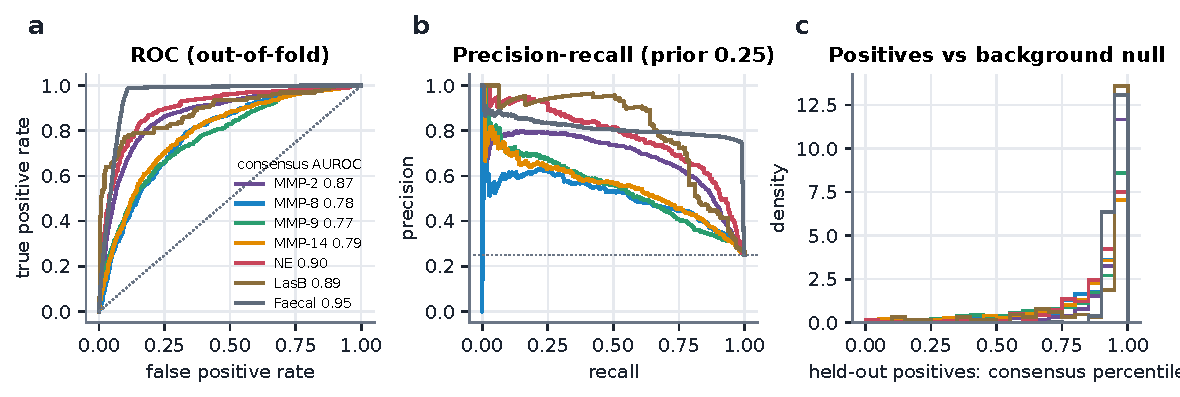
\includegraphics[width=\textwidth]{../figures/F09_roc_pr.pdf}
  \caption{Out-of-fold performance of the consensus score. \textbf{A:} ROC
    curves. \textbf{B:} precision-recall curves. \textbf{C:} distribution of the
    consensus percentile of held-out positives, which concentrates near the top
    of the background distribution for every protease.}
  \label{fig:roc}
\end{figure}

\subsection{Results: model and representation comparison}

Seven models were compared on identical folds: a constant prior, a
composition-only logistic regression, one-hot and VHSE logistic regressions, the
PSSM, and gradient-boosted trees on both encodings. Three conclusions follow.

\begin{itemize}[leftmargin=*,noitemsep]
\item \textbf{Position matters and composition mostly does not.} For six of
  seven proteases composition alone gives $0.60$--$0.74$ AUROC and the VHSE
  model exceeds it significantly; label-shuffled controls give
  \shuffleMin--\shuffleMax{}. LasB is the exception: composition alone reaches
  $0.886$, statistically indistinguishable from the full model. The LasB model
  therefore detects largely elastin-like composition, as expected from a
  positive set that is $76\%$ elastin \CONF.
\item \textbf{No strong position--position interaction is evident.}
  Gradient-boosted trees reach within $0.013$ AUROC of the better of the one-hot
  regression and the PSSM on every protease and exceed it only on NE, by $0.007$
  \CONF.
\item \textbf{The representation trade-off is real.} On data-rich proteases
  (MMP-2, MMP-8) the one-hot regression and the PSSM exceed the VHSE model
  significantly, by $0.017$ to $0.034$ AUROC, consistent with the bias measured
  by the subspace coverage below. On NE and LasB the VHSE model exceeds the
  one-hot regression significantly ($+0.021$ and $+0.033$). The learning curves
  show the same crossover: VHSE leads at small training sizes and is overtaken
  as data grow \CONF.
\end{itemize}

The PSSM has no fitted hyperparameter and lies at or within the interval of the
best model for every protease, which is the reason the shipped score combines it
with the logistic regression.

\begin{center}
\small\renewcommand{\arraystretch}{1.25}
\begin{tabular}{@{}lccccccc@{}}\toprule
Protease & Prior & Composition & One-hot LR & VHSE LR & PSSM & One-hot GBM & VHSE GBM \\\midrule
MMP-2 & 0.500 & 0.664 & 0.871 & 0.854 & \textbf{0.874} & 0.869 & 0.872 \\
MMP-8 & 0.500 & 0.596 & 0.777 & 0.750 & \textbf{0.784} & 0.780 & 0.783 \\
MMP-9 & 0.500 & 0.639 & 0.756 & 0.754 & \textbf{0.761} & 0.752 & 0.755 \\
MMP-14 & 0.500 & 0.633 & 0.772 & 0.771 & \textbf{0.785} & 0.773 & 0.779 \\
Neutrophil elastase & 0.500 & 0.676 & 0.866 & 0.887 & 0.885 & 0.892 & \textbf{0.894} \\
LasB & 0.500 & 0.886 & 0.845 & 0.877 & 0.881 & 0.878 & \textbf{0.889} \\
Faecal serine proteases & 0.500 & 0.742 & 0.952 & 0.951 & \textbf{0.953} & 0.950 & 0.951 \\
\bottomrule\end{tabular}

\end{center}

The table gives cross-validated AUROC by model (bold: best); the prior gives
$0.5$. The next table gives the AUROC of each alternative minus that of the VHSE
logistic regression under a paired cluster bootstrap (asterisk: $95\%$ interval
excludes zero).

\begin{center}
\small\renewcommand{\arraystretch}{1.25}
\begin{tabular}{@{}lcccc@{}}\toprule
Protease & One-hot LR & PSSM & One-hot GBM & VHSE GBM \\\midrule
MMP-2 & +0.017$^{*}$ & +0.020$^{*}$ & +0.015$^{*}$ & +0.018$^{*}$ \\
MMP-8 & +0.027$^{*}$ & +0.034$^{*}$ & +0.029$^{*}$ & +0.034$^{*}$ \\
MMP-9 & +0.003 & +0.008 & -0.002 & +0.001 \\
MMP-14 & +0.000 & +0.014$^{*}$ & +0.002 & +0.009 \\
Neutrophil elastase & -0.021$^{*}$ & -0.002 & +0.005 & +0.007 \\
LasB & -0.033$^{*}$ & +0.003 & +0.000 & +0.011 \\
Faecal serine proteases & +0.000 & +0.001 & -0.001 & -0.000 \\
\bottomrule\end{tabular}

\end{center}

\begin{figure}[H]
  \centering
  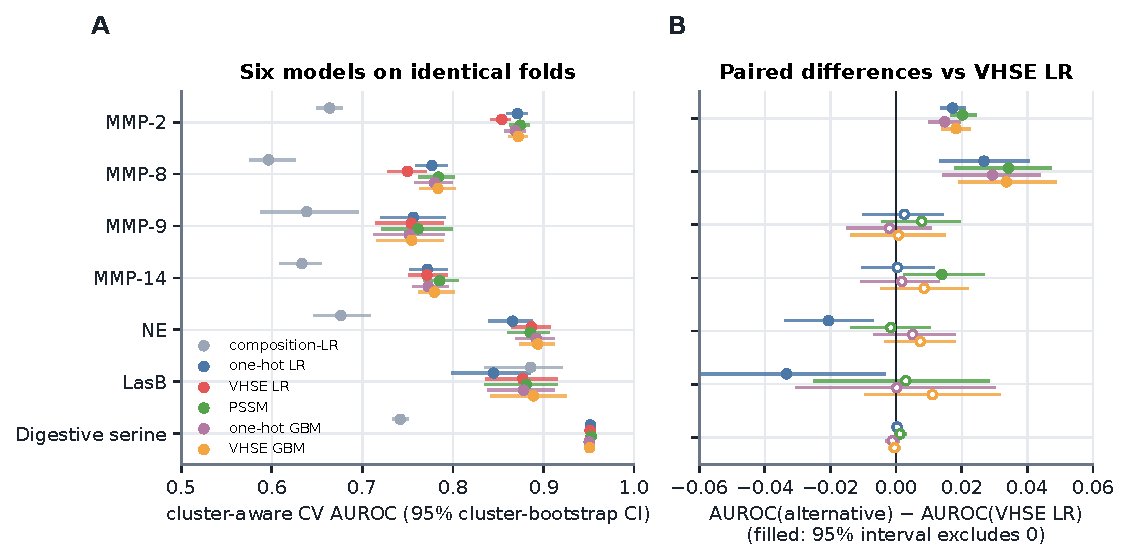
\includegraphics[width=\textwidth]{../figures/F05_model_comparison.pdf}
  \caption{\textbf{A:} cluster-aware AUROC of six models on identical folds with
    $95\%$ cluster-bootstrap intervals. \textbf{B:} paired difference
    (alternative minus VHSE logistic regression); filled markers have intervals
    excluding zero. The composition-only model lies $0.12$--$0.21$ below for every
    protease except LasB and is omitted from panel B for scale.}
  \label{fig:models}
\end{figure}

\begin{figure}[H]
  \centering
  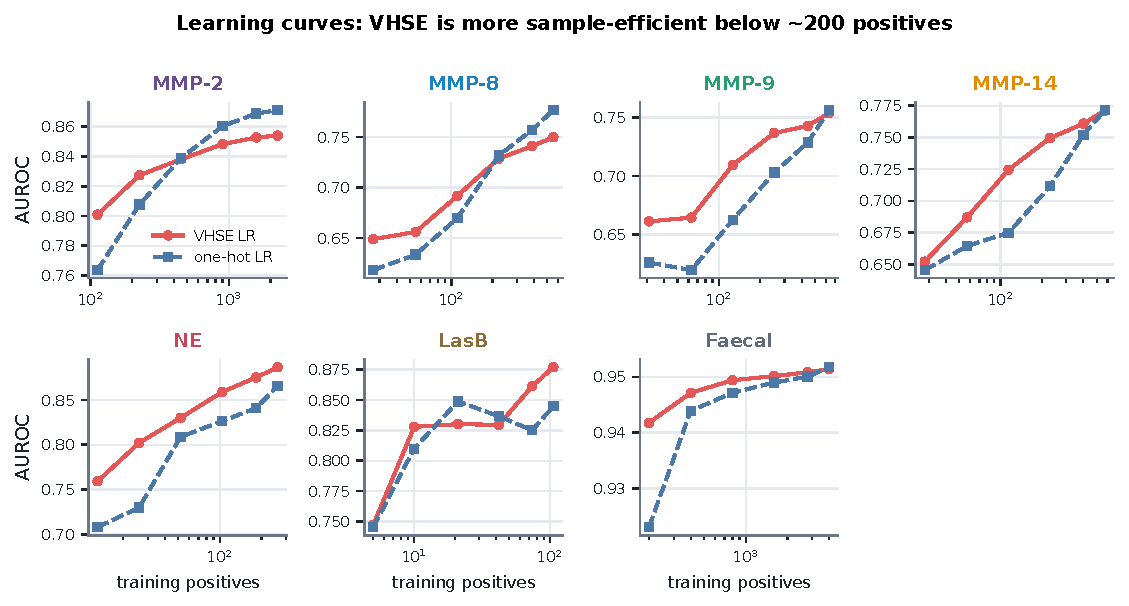
\includegraphics[width=\textwidth]{../figures/F06_learning_curves.pdf}
  \caption{Learning curves: AUROC as a function of the number of training
    positives for the VHSE and one-hot logistic regressions.}
  \label{fig:lc}
\end{figure}

\subsection{Results: training against other proteases}

Three negative-set designs were compared on a common held-out test set within
identical folds: composition-shuffled positives plus background (the earlier
design), background only, and the panel design of Part~\ref{sec:data}. Each was
scored on held-out target positives against background windows and against
held-out positives of the other proteases. The panel design costs
$0.01$--$0.02$ AUROC against background and gains against competitors on every
protease, most where it matters: for LasB from $0.80$ (background only) and
$0.68$ (shuffled) to $0.86$, for MMP-14 from $0.65$ to $0.73$, and for MMP-2
from $0.76$ to $0.79$ \CONF.

\begin{center}
\small\renewcommand{\arraystretch}{1.25}
\begin{tabular}{@{}lcccccc@{}}\toprule
 & \multicolumn{2}{c}{Shuffled + background} & \multicolumn{2}{c}{Background only} & \multicolumn{2}{c}{Panel (ours)} \\
\cmidrule(lr){2-3}\cmidrule(lr){4-5}\cmidrule(lr){6-7}
Protease & vs bkg & vs comp. & vs bkg & vs comp. & vs bkg & vs comp. \\\midrule
MMP-2 & 0.881 & 0.756 & 0.885 & 0.762 & 0.882 & 0.787 \\
MMP-8 & 0.834 & 0.654 & 0.828 & 0.651 & 0.810 & 0.683 \\
MMP-9 & 0.819 & 0.660 & 0.832 & 0.667 & 0.816 & 0.683 \\
MMP-14 & 0.831 & 0.660 & 0.833 & 0.649 & 0.811 & 0.727 \\
Neutrophil elastase & 0.850 & 0.910 & 0.852 & 0.900 & 0.848 & 0.926 \\
LasB & 0.801 & 0.676 & 0.889 & 0.798 & 0.891 & 0.863 \\
Faecal serine proteases & 0.954 & 0.939 & 0.954 & 0.938 & 0.953 & 0.944 \\
\bottomrule\end{tabular}

\end{center}

\begin{figure}[H]
  \centering
  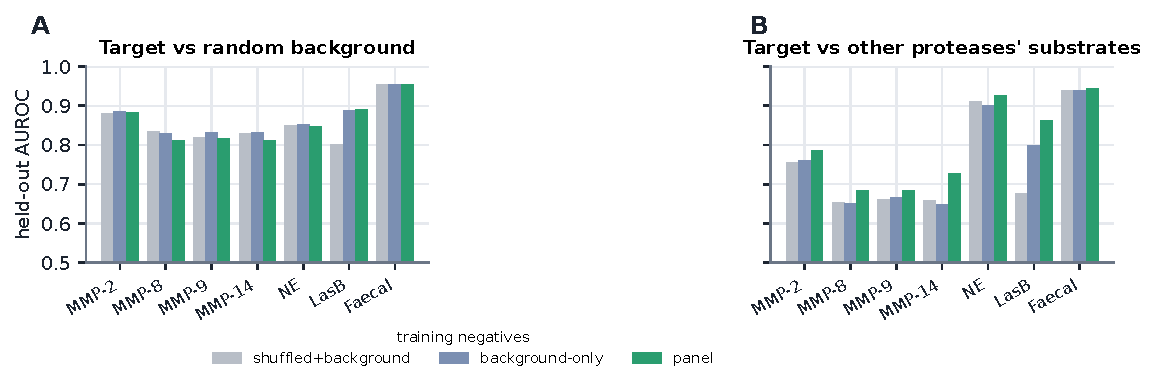
\includegraphics[width=\textwidth]{../figures/F07_negative_design.pdf}
  \caption{Effect of the training negatives on detection (\textbf{A}) and
    cross-protease discrimination (\textbf{B}).}
  \label{fig:neg}
\end{figure}

\subsection{Results: regularisation, leakage and controls}

Choosing $C$ by inner cross-validation raises or matches the $C=1$ default,
selecting $C=0.01$--$0.1$ for every protease except the faecal group. Random and
cluster-aware folds differ by at most \maxLeakGap{} AUROC, so near-duplicate
leakage is not a material source of optimism in these data, although the folds
guard against it. The table gives regularisation (AUROC at $C=1$ against nested
selection), fold construction (random against clustered, fixed $C=0.1$), the
label-shuffle control (mean of five permutations), and the variance-weighted
share of the learned PSSM log-odds that lies inside the VHSE subspace.

\begin{center}
\small\renewcommand{\arraystretch}{1.25}
\begin{tabular}{@{}lcccccc@{}}\toprule
 & \multicolumn{2}{c}{Regularisation} & \multicolumn{2}{c}{Fold construction} & Label & VHSE span \\
\cmidrule(lr){2-3}\cmidrule(lr){4-5}
Protease & $C=1$ & nested & random & clustered & shuffle & coverage \\\midrule
MMP-2 & 0.854 & 0.854 & 0.855 & 0.854 & 0.505 & 79\% \\
MMP-8 & 0.750 & 0.755 & 0.752 & 0.752 & 0.493 & 64\% \\
MMP-9 & 0.754 & 0.760 & 0.755 & 0.756 & 0.493 & 64\% \\
MMP-14 & 0.771 & 0.772 & 0.771 & 0.773 & 0.509 & 79\% \\
Neutrophil elastase & 0.887 & 0.895 & 0.897 & 0.895 & 0.495 & 65\% \\
LasB & 0.877 & 0.877 & 0.886 & 0.879 & 0.526 & 65\% \\
Faecal serine proteases & 0.951 & 0.951 & 0.951 & 0.951 & 0.494 & 77\% \\
\bottomrule\end{tabular}

\end{center}

\begin{figure}[H]
  \centering
  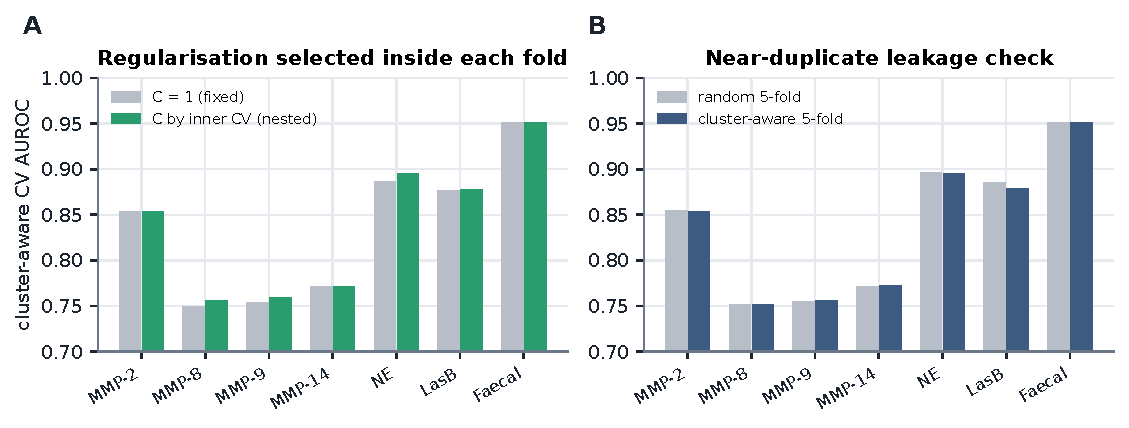
\includegraphics[width=\textwidth]{../figures/F08_tuning_and_leakage.pdf}
  \caption{\textbf{A:} nested regularisation selection against fixed $C=1$.
    \textbf{B:} random against cluster-aware folds.}
  \label{fig:tune}
\end{figure}

\subsection{Results: calibration and scale}

Reliability curves of the logistic-regression score lie below the diagonal:
with balanced class weights the score is a posterior under a $50{:}50$ prior,
whereas the training mixture has a positive prior of $0.25$ and real sequences a
far lower one. Expected calibration error is $0.06$--$0.20$. Base rates also
differ by model, the mean score on random windows ranging from $0.11$ (faecal
group) to $0.35$ (MMP-14), which motivates the percentile scale of
Part~\ref{sec:panel} \CONF.

\begin{figure}[H]
  \centering
  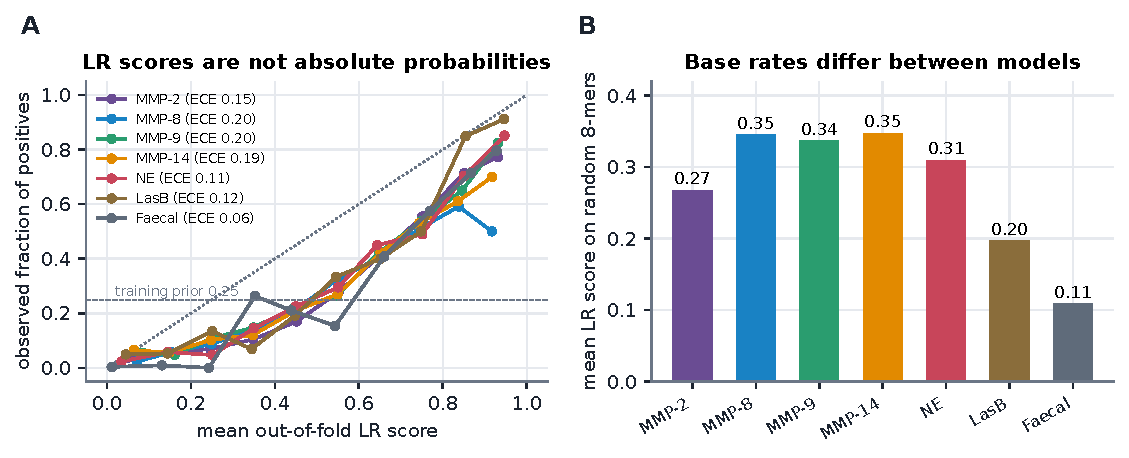
\includegraphics[width=\textwidth]{../figures/F10_calibration.pdf}
  \caption{\textbf{A:} reliability curves of the out-of-fold
    logistic-regression score. \textbf{B:} mean logistic-regression score on
    random background windows for each final model.}
  \label{fig:calib}
\end{figure}

\subsection{Results: selectivity between proteases}

The next table gives, for each target model, the held-out AUROC for separating
the target's substrates from a competitor's substrates (the competitor's windows
were training negatives, but each is scored out-of-fold). The NE and faecal
models separate their substrates from every competitor's at $0.90$--$0.98$. The
MMP models separate theirs from NE's at $0.89$--$0.93$, but from LasB's and the
faecal group's at only $0.63$--$0.89$. Within the MMP family discrimination is
modest ($0.53$--$0.72$), lowest for MMP-14 against MMP-2 ($0.53$) and MMP-8 against
MMP-2 ($0.57$) \CONF.

\begin{center}
\small\renewcommand{\arraystretch}{1.25}
\begin{tabular}{@{}lccccccc@{}}\toprule
Target model & MMP-2 & MMP-8 & MMP-9 & MMP-14 & NE & LasB & Faecal \\\midrule
MMP-2 & -- & 0.72 & 0.68 & 0.69 & 0.93 & 0.79 & 0.89 \\
MMP-8 & 0.57 & -- & 0.58 & 0.64 & 0.91 & 0.82 & 0.63 \\
MMP-9 & 0.59 & 0.65 & -- & 0.70 & 0.90 & 0.63 & 0.63 \\
MMP-14 & 0.53 & 0.62 & 0.70 & -- & 0.89 & 0.80 & 0.84 \\
Neutrophil elastase & 0.93 & 0.93 & 0.93 & 0.94 & -- & 0.92 & 0.96 \\
LasB & 0.84 & 0.90 & 0.81 & 0.84 & 0.87 & -- & 0.91 \\
Faecal & 0.96 & 0.90 & 0.91 & 0.96 & 0.98 & 0.97 & -- \\
\bottomrule\end{tabular}

\end{center}

\begin{figure}[H]
  \centering
  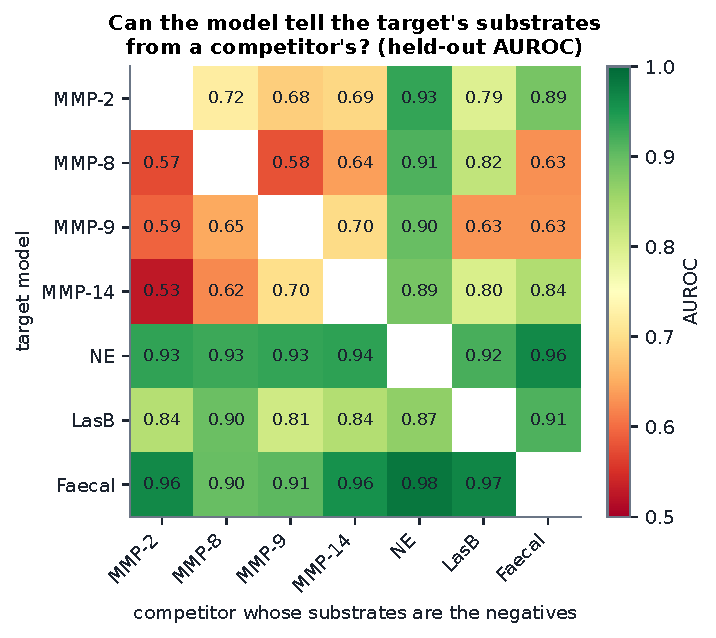
\includegraphics[width=0.62\textwidth]{../figures/F11_selectivity_matrix.pdf}
  \caption{Cross-protease discrimination matrix (data of the preceding table).}
  \label{fig:selmat}
\end{figure}

A low competitor AUROC does not by itself indicate a poor model. By
Eq.~\eqref{eq:contam}, if a fraction $\pi$ of a competitor's substrates are also
cleaved by the target, the measured AUROC is at most $1-\pi/2$ for a perfect
model. Exact-window overlap between protease positive sets is small, but the MMPs
share their dominant preferences \cit{1}, so many competitor windows are
plausibly cleaved by the target as well; the ceiling for MMP-against-MMP AUROC is
therefore below $1$ by an amount that sequence data alone cannot measure
\FLAG. The practical conclusion is unchanged: from a P4--P4$'$ window alone the
MMPs cannot be reliably distinguished, and a sensor design should not depend on
it.

\begin{figure}[H]
  \centering
  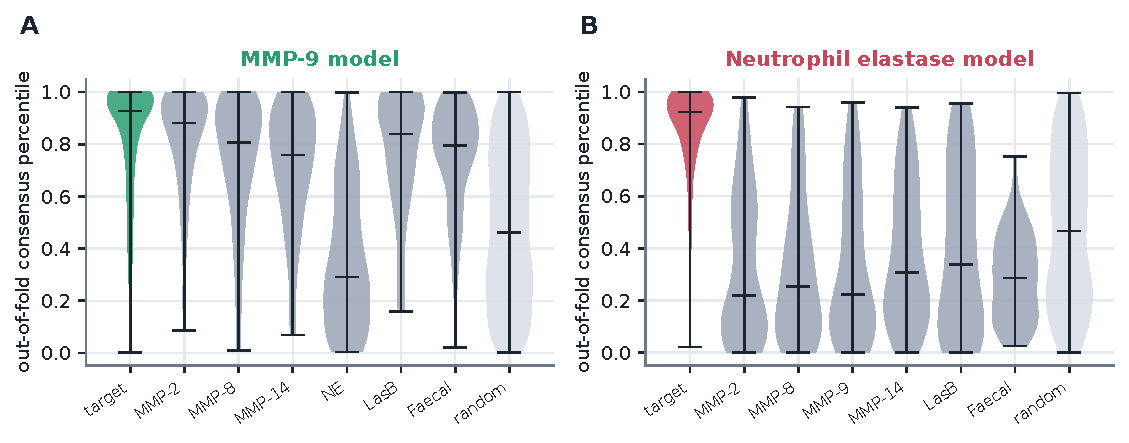
\includegraphics[width=\textwidth]{../figures/F16_score_distributions.pdf}
  \caption{Out-of-fold consensus percentiles of held-out positives (target) and
    of each competitor's substrates and random windows for the MMP-9 model
    (\textbf{A}) and the NE model (\textbf{B}). The MMP-9 model places MMP-2 and
    MMP-8 substrates almost as high as its own; the NE model separates them
    sharply.}
  \label{fig:dist}
\end{figure}

\subsection{Results: what the models learned}

Coefficient stability by cluster bootstrap identifies which learned effects are
reliable: between $17$ (MMP-14) and $35$ (MMP-2) of the $64$ standardised
coefficients per model have $95\%$ intervals excluding zero, so the
position-level pattern is more trustworthy than any single descriptor weight.
Total contribution is concentrated at $\pos{3}$ and $\prm{1}$ for the MMPs, at
$\pos{1}$ for NE and the faecal group, and is spread across positions for LasB;
the electronic family, which accounts for four of the eight descriptors, carries
the largest share for every protease.

\begin{figure}[H]
  \centering
  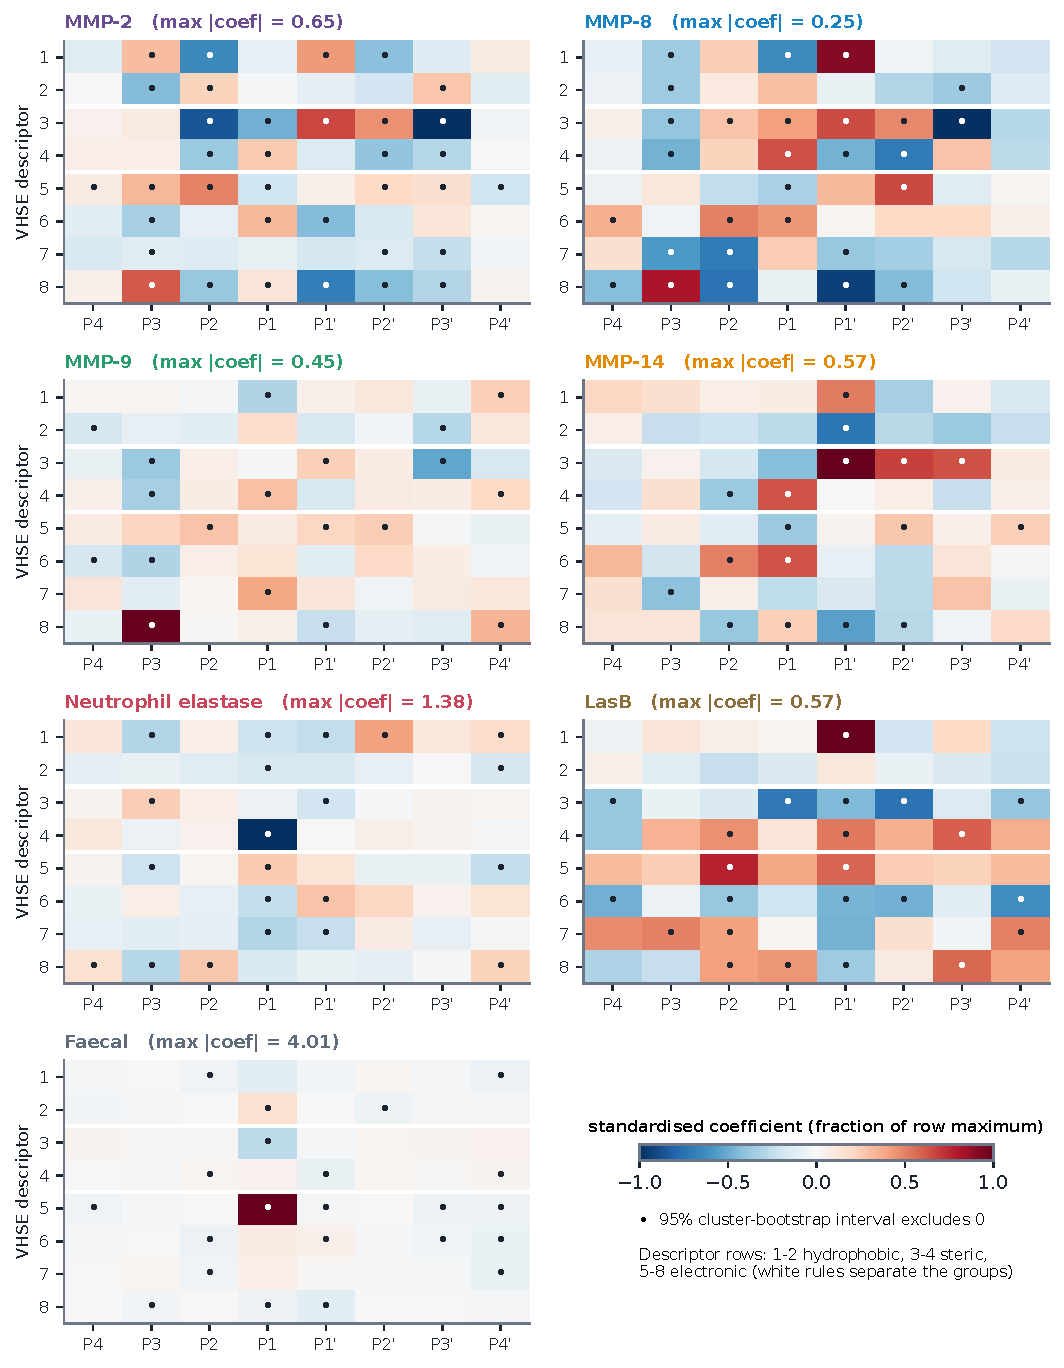
\includegraphics[width=0.97\textwidth]{../figures/F12_coefficients.pdf}
  \caption{Standardised logistic-regression coefficients by position and VHSE
    descriptor. Dots mark coefficients whose $95\%$ cluster-bootstrap interval
    excludes zero. Colours are scaled to each protease's largest coefficient.}
  \label{fig:coef}
\end{figure}

\begin{figure}[H]
  \centering
  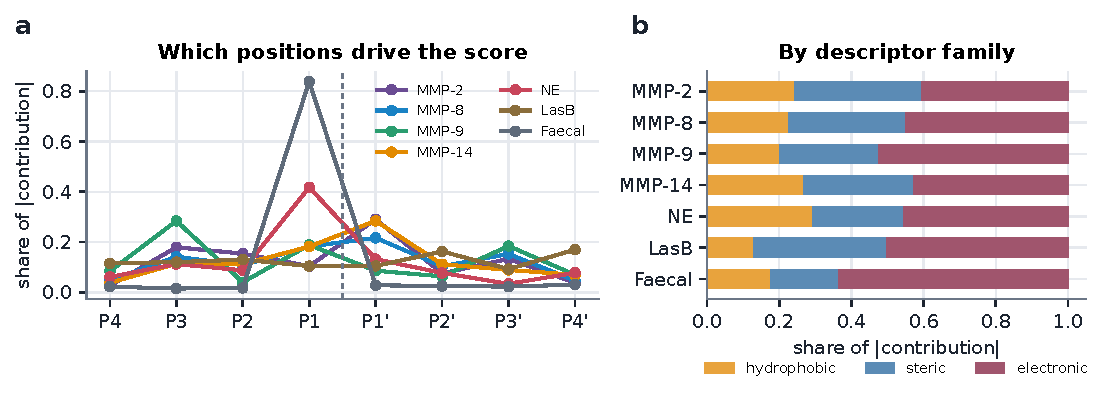
\includegraphics[width=\textwidth]{../figures/F13_position_importance.pdf}
  \caption{\textbf{A:} share of mean absolute logit contribution by position,
    computed on training positives. \textbf{B:} share by descriptor family.}
  \label{fig:pos}
\end{figure}
